\documentclass[12pt]{article}
 
\usepackage[landscape,margin=0.5in,top=0.5in,bottom=0.5in,a4paper]{geometry}
\usepackage{amsmath,multicol,titlesec,graphicx,listings}

\usepackage[utf8]{inputenc}
\titlespacing{\section}{0pt}{5pt}{0pt}
\titlespacing{\subsection}{0pt}{5pt}{0pt}
\titlespacing{\subsubsection}{0pt}{5pt}{0pt}
\setlength{\parindent}{0pt}
\pagenumbering{gobble}
\titleformat*{\section}{\large\bfseries}
\titleformat*{\subsection}{\bfseries}
\setlength{\columnseprule}{1pt}
 
\begin{document}
\raggedright
\begin{multicols}{4}

\subsection{Condensadors}

\underline{Capacitat} $\varepsilon \varepsilon_0 A / d$ \\
\underline{Càrrega} $q = CV$ \\
\underline{Energia electroestàtica}: $W = E = \frac{1}{2}CV_C^2 = \frac{1}{2}\frac{Q^2}{C}$






\underline{Nombre d'Avogadro}: $N_A = 6,22 \times 10^{23}$ \\
\underline{Eq. de Shockley}: $I = I_0 \left( e^{\frac{V}{\eta V_\tau}} -1 \right)$ \\
$V_\tau = \frac{k_BT}{e}, \eta \approx 1 $ \\
\underline{Eq. de Plank}: $E = h \nu$ \\
$h = 6,62 \times 10^{-34}$ [Js] \\

\section{Transistors}

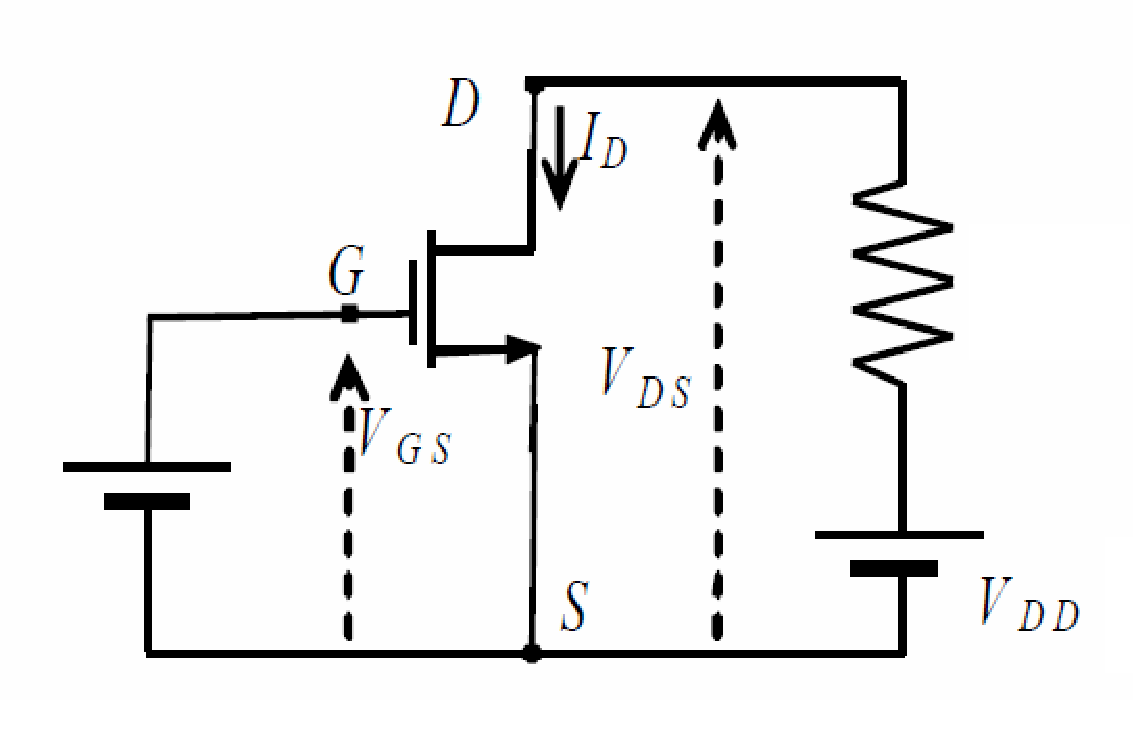
\includegraphics[width=\linewidth]{Figures/Figura1.pdf}

\subsection{Transistors NMOS}

\texttt{if ($V_{GS} > V_T$) }\\
\texttt{ if ($V_{DS} > V_{GS} - V_T$) (1)} \\
\texttt{ else (2)} \\
\texttt{else (3)} \\
\texttt{ } \\
(1) \underline{zona de saturació}: $I_D = \frac{\beta}{2} (V_{GS}-V_T)^2$ \\
(2) \underline{zona lineal (óhmica)}: $\beta \left[ \left( V_{GS} - V_T \right) V_{DS} - \frac{V_{DS}^2}{2} \right]$ \\
(3) \underline{zona de tall}: $I_D = 0$ \\

\subsection{Transistors PMOS}

\texttt{if ($V_{GS} < V_T$) }\\
\texttt{ if ($V_{DS} < V_{GS} - V_T$) (1)} \\
\texttt{ else (2)} \\
\texttt{else (3)} \\
\texttt{ } \\
(1) \underline{zona de saturació}: $I_D = \frac{\beta}{2} (V_{GS}-V_T)^2$ \\
(2) \underline{zona lineal (óhmica)}: $\beta \left[ \left( V_{GS} - V_T \right) V_{DS} - \frac{V_{DS}^2}{2} \right]$ \\
(3) \underline{zona de tall}: $I_D = 0$ \\

\section{Retras i potència en circuits digitals}

Interruptor de: \\
\qquad càrrega $C \approx 1 [F]$ \\
\qquad tensió d'alimentació $V_{DD}$ \\
\qquad relació d'activitat $p$ \\
\qquad corrent $I$ \\
\qquad clock $f_C$ \\
\underline{Potència dinàmica de càrrega}: $P_{\text{dinàmica}} = p f_C C V_{DD}^2$ \\
\underline{Potència estàtica}: $P_{\text{estàtica}} = I V_{DD}$ \\
\underline{Potència dissipada}: $P = P_{\text{dinàmica}} + P_{\text{estàtica}}$ \\
\underline{Energia de commutació}: $E = C V_{DD}^2 + \frac{I V_{DD}}{p f_C}$ \\








\section{Circuits RC}

\underline{Càrrega}: $q(t) = VC\left( 1 - e^{-\frac{t}{\tau_C}}\right)$, $I(t) = \frac{\varepsilon}{R} e^{-\frac{t}{\tau_C}}$ \\
\underline{Descàrrega}: $q(t) = VCe^{-\frac{t}{\tau_C}}$, $I(t) = -\frac{V}{R}e^{-\frac{t}{\tau_C}}$ \\

$\tau_C = RC$
\subsection{Condensadors}

\underline{Capacitat} $\varepsilon \varepsilon_0 A / d$ \\
\underline{Càrrega} $q = CV$ \\
\underline{Energia electroestàtica}: $W = E = \frac{1}{2}CV_C^2 = \frac{1}{2}\frac{Q^2}{C}$

\section{Circuits RL}
\underline{Càrrega}: $I(t) = \frac{\varepsilon}{R_{\text{est}}} \left(1 - e^{-\frac{t}{\tau_L}}\right)$ \\
\underline{Descàrrega}: $I(t) = \frac{V}{R_{\text{est}}}e^{-\frac{t}{\tau_L}}$ \\
$\tau_L = \frac{L}{R}, R_{\text{est}} = R + r$

\subsection{Solenoides}

\underline{Energia} $U = \frac{1}{2} L I^2$ \\ 
\underline{Flux}: $\Phi = NBS = \frac{\mu_0 N^2SI}{l}$ \\
\underline{Coeficient d'autoinducció}: $L = \frac{\Phi}{I} = \frac{\mu_0N^2S}{l}$ \\
$\varepsilon_L= -\frac{\text{d}\Phi}{\text{d}t} = -L \frac{\text{d}I}{\text{d}t}$

\section{Corrent alterna}

\underline{f.e.m. alterna}: $V(t) = V_0\text{cos}(\omega t+\varphi)$, $T = \frac{2\pi}{\omega}$, $I(t) = \frac{V(t)}{R} = \frac{V_0}{R}\text{cos}(\omega t + \varphi) = I_0\text{cos}(\omega t + \varphi)$ \\
\underline{Flux}: $\Phi = BSN\text{cos}(\omega t+\theta)$, $B$ camp magnètic \\
\underline{Llei Faraday}: $\varepsilon(t) = V_0\text{sin}(\omega t + \theta_0)$ \\
\underline{Voltatge eficaç}: $V_{\text{ef}} = \frac{V_0}{\sqrt{2}}$ \\
\underline{Intensitat eficaç}: $I_{\text{ef}} = \frac{I_0}{\sqrt{2}}$

\subsection{Circuit amb condensador}

\underline{Voltatge}: $V(t) = V_0\text{cos}(\omega t)$ \\
\underline{Intensitat}: $I(t) = -V_0\omega C \text{sin}(\omega t) = -I_0\text{sin}(\omega t)$ $= I_0\text{cos}(\omega t + \frac{\pi}{2})$ (desfase de $-\frac{\pi}{2}$) \\
$V(t) = V_0 e^{i\omega t}$, $\implies I(t) = V_0i\omega Ce^{i\omega t}$ \\
\underline{Llei d'Ohm}: $(V=IR_C)$, $R_C = \frac{1}{i\omega C}, [C] = F$ \\
\underline{Reactancia capacitiva}: $X_C = \vert R_C\vert = \frac{1}{\omega C}$, $R_C = \frac{X_C}{i} = -iX_C$

\subsection{Circuit amb inducció}

\underline{Voltatge}: $V(t) = V_0\text{cos}(\omega t)$ \\
\underline{Autoinducció a la bobina}: $\varepsilon_L = -L \frac{\text{d}I}{\text{d}t}$ \\
\underline{Segona llei Kirchhoff}: $V(t) + \varepsilon_L = 0 \implies I(t) = \frac{V_0}{L\omega}\text{sin}(\omega t) = I_0\text{cos}(\omega t - \frac{\pi}{2})$ (desfase de $\frac{\pi}{2}$) \\
$V(t) = V_0e^{i\omega t}$, $\implies I = \frac{V_0}{i\omega L}e^{i\omega t}$ \\
\underline{Llei d'Ohm}: $V=IR_L$, $R_L=i\omega L, [L] = H$ \\
\underline{Reactancia inductiva}: $X_L = \vert R_L\vert = \omega L$, $R_L = iX_L$

\section{Impedància. Llei d'Ohm}

\underline{Llei d'Ohm}: $V = IZ$ \\
\underline{Impedància}: $\bar{Z} = R + iX \begin{cases} \text{Resistència: } R \\ \text{Condensador: } -iX_C \\ \text{Inducció: } iX_L \end{cases}$

\subsection{Circuit LCR}

\underline{Angle de fase}: tg$(\varphi)=\frac{X_L-X_C}{R}, ("I" + \varphi = "V")$ \\
\underline{Corrent máxim}: $I_0 = \frac{\varepsilon_0}{Z}$ \\
\underline{Freqüència}: $f = \frac{\omega}{2\pi}$ \\
\underline{Ressonància}: $Z = \text{Re}[Z] \implies \omega^2 = \frac{1}{LC}$

\section{Potència}

\underline{Potència instantània}: $P(t) = V(t)I(t) = V_0I_0\text{cos}(\omega t)\text{cos}(\omega t - \varphi)$ \\
\underline{Potència mitja}: $\frac{V_0I_0}{2\text{cos}(\varphi)} = V_\text{ef}I_\text{ef}\text{cos}(\varphi)$

\subsection{Potència en una resistència}

\underline{No desfase}: $\varphi = 0, V(t) = V_0\text{cos}(\omega t), I(t) = I_0\text{cos}(\omega t)$ \\
\underline{Potència instanània}: $P(t) = V_0\text{cos}(\omega t)I_0\text{cos}(\omega t) = \frac{V_0^2}{R}\text{cos}^2(\omega t)$ \\
\underline{Potència mitja}: $P = \frac{V_0^2}{2R}$ \\
\underline{Valors eficaços}: $V_{\text{ef}} = \frac{V_0}{\sqrt{2}}$, $I_{\text{ef}} = \frac{I_0}{\sqrt{2}}$ \\
\underline{Potència dissipada}: $P = \frac{V_{\text{ef}}^2}{R} = RI_{\text{ef}}^2$

\subsection{Potència en un condensador}

\underline{Desfase}: $\varphi = -\frac{\pi}{2}, V(t) = V_0\text{cos}(\omega t), I(t) = I_0\text{cos}(\omega t + \frac{\pi}{2}) = -I_0\text{sin}(\omega t)$ \\
\underline{Potència instantània}: $P(t) = -\frac{V_0^2}{X_C}\text{sin}(\omega t)\text{cos}(\omega t) = -\frac{V_0^2}{2X_C}\text{sin}(2\omega t)$ \\
\underline{Potència mitja}: 0

\subsection{Potència en una inducció}

\underline{Desfase}: $\varphi = \frac{\pi}{2}, V(t) = V_0\text{cos}(\omega t), I(t) = I_0\text{cos}(\omega t - \frac{\pi}{2}) = I_0\text{sin}(\omega t)$ \\
\underline{Potència instantània}: $P(t) = \frac{V_0^2}{X_L}\text{sin}(\omega t)\text{cos}(\omega t) = \frac{V_0^2}{2X_L}\text{sin}(2\omega t)$ \\
\underline{Potència mitja}: 0

\subsection{Potència complexa}

$\bar{V} = V_0e^{i\omega t}, \bar{I} = I_0e^{i(\omega t - \varphi)}, \bar{Z} = Z e^{i\varphi}$ \\
\underline{Potència complexa}: $\bar{S} = \frac{\bar{V}\bar{I}^*}{2} = \frac{V_0e^{i\omega t}I_0e^{-i(\omega t - \varphi)}}{2} = \frac{V_0I_0}{2}e^{i\varphi} = V_{\text{ef}}I_{\text{ef}}(\text{cos}(\varphi) + i\text{ sin}(\varphi))$ \\
\underline{Potència activa [W]}: $P = \text{Re}[\bar{S}] = V_{\text{ef}}I_{\text{ef}}\text{cos}(\varphi)$ \\
\underline{Potència reactiva [VA]}: $Q = \text{Im}[\bar{S}] = V_{\text{ef}}I_{\text{ef}}\text{sin}(\varphi)$ \\
\underline{Potència aparent [VA]}: $S = \vert \bar{S} \vert = V_{\text{ef}}I_{\text{ef}}$

\subsection{Factor de potència}

\underline{Factor de potència}: $\text{cos}(\varphi) = \frac{P}{S}$ \\
\underline{Millora del f.d.p. en sèrie}: $Z = R + iX$, connectem $X' = -X$. $(X>0,\varphi>0) \implies C=\frac{1}{\omega X}, (X<0, \varphi<0) \implies L=\frac{\vert X\vert}{\omega}$ \\
\underline{Millora del f.d.p. en paral·lel}: $X' = -\frac{(R^2+X^2)}{X} = -\frac{\vert Z\vert}{\text{sin}(\varphi)}$

\section{Superposició de senyals. Amplada de banda}

\underline{Senyal sinusoidal}: $F(t) = A\text{sin}(2\pi f_1t+ \varphi)$ \\
\underline{Espectre}: Rang de freqüències del senyal. \\
%\underline{Amplada de banda ($f_b$)}: Mida del espectre. \\
\underline{Freqüència $n$-èssima} \underline{harmònica}: $f_n = \frac{n\omega_0}{2\pi} = \frac{n}{T}$ \\
\underline{Pols}: Un cicle. \\
\underline{Velocitat de transmissió} \underline{màxima}: $v_\text{max} = \frac{1}{T_\text{bit}} = \frac{1}{2\tau} = \frac{f_b}{2}, T_{\text{bit}} = 2 \tau$ \\
\end{multicols}
\end{document}
